\documentclass{article}

\usepackage[latin1]{inputenc}
\usepackage{pgfplots}
\usepackage{tikz}

\pgfplotsset{compat=1.10}

\begin{document}
\pagestyle{empty}

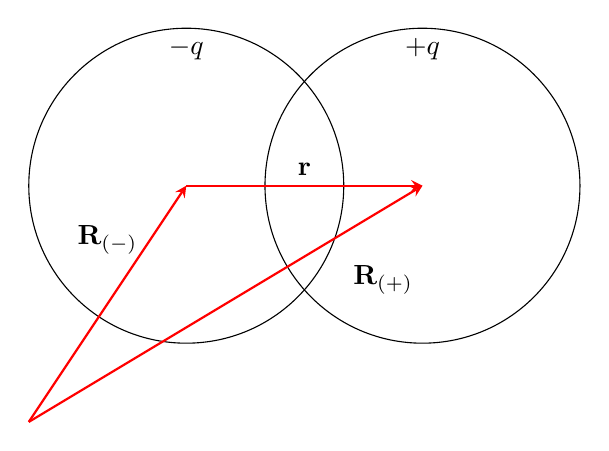
\begin{tikzpicture}[>=stealth]
	\draw[thin] (0, 0) circle [radius=2];
	\draw[thin] (3, 0) circle [radius=2];

	\draw[-latex, red, thick, ->] (0, 0) -- (3, 0);
	\node[above] at (1.5, 0) {$\textbf{r}$};

	\draw[-latex, red, thick, ->] (-2, -3) -- (0, 0);
	\node[above] at (-1, -1) {$\textbf{R}_{(-)}$};

	\draw[-latex, red, thick, ->] (-2, -3) -- (3, 0);
	\node[above] at (2.5, -1.5) {$\textbf{R}_{(+)}$};

	\node[below] at (0, 2) {$-q$};
	\node[below] at (3, 2) {$+q$};
\end{tikzpicture}


\end{document}